\documentclass[12pt,a4paper,oneside]{book}

\usepackage[titletoc]{appendix}
\usepackage{subfigure}
\usepackage{pgfplots}
\usepackage{booktabs}
\usepackage{algorithm}
\usepackage{algpseudocode}
%\usepackage{algorithmic}
\usepackage{amsmath}
\usepackage{graphics}
\usepackage{epsfig}
% border setting
\usepackage[ top=2.5cm,bottom=2.5cm,left=2.5cm,right=2.5cm ]{ geometry }

% The default for LaTeX is to have no indent after sectional headings, like \chapter and \section. ()
\usepackage{indentfirst}

% http://tex.stackexchange.com/questions/28333/continuous-v-per-chapter-section-numbering-of-figures-tables-and-other-docume
\usepackage{chngcntr}
\counterwithout{figure}{chapter}
\counterwithout{table}{chapter}

% This prevents placing floats before a section
\usepackage[section]{placeins}
\let\Oldsubsection\subsection
\renewcommand{\subsection}{\FloatBarrier\Oldsubsection}

% source code hightlighting
\usepackage{listings}
\lstset{
  numbers=left,
  stepnumber=1,
  firstnumber=1,
  captionpos=b,
  tabsize=2,
  basicstyle=\small,
  numberfirstline=true
}

% setting the page number to footer
\usepackage{fancyhdr}
\fancyhf{}
\cfoot{\thepage}
\pagestyle{fancy}
% no header and footer bar
\renewcommand{\headrulewidth}{0pt}
\renewcommand{\footrulewidth}{0pt}

% setup bibliography
\usepackage[sorting=none,backend=bibtex]{biblatex}
\addbibresource{reference.bib}

% line height setting
\linespread{1.5}
\usepackage{setspace}

% Graphics settings
\usepackage{graphicx}
\graphicspath{ {./figures/} }

\usepackage{background}
\newcommand\DeactivateBG{\backgroundsetup{contents={}}}
\newcommand\ActivateBG{
  \backgroundsetup{
      contents={
\includegraphics[]{logo.jpg}},
      scale=1,
      opacity=0.4,
      angle=0
  }
}

\usepackage{comment}

% do not place figure at the middle of a empty page
\makeatletter
\setlength{\@fptop}{0pt}
\makeatother

% Chinese typesetting
\usepackage{xeCJK}
%\setCJKmainfont{SourceHanSansTW-Light.otf}
\setCJKmainfont[
  BoldFont={SourceHanSansTW-Normal.otf},
  ItalicFont={SourceHanSansTW-Light.otf}
]{SourceHanSansTW-Light.otf}
\newcommand{\myHuge}[1]{\fontsize{40}{50} #1}

\newcommand{\chineseTitle}{基於蒙地卡羅樹搜尋法之路徑探索於符號執行}
\newcommand{\englishTitle}{MCTS-based Path Exploration for Symbolic Execution}

\newcommand{\studentCnName}{葉家郡}
\newcommand{\studentEnName}{Jia-Jun Yeh}
\newcommand{\advisorCnName}{黃世昆}
\newcommand{\advisorEnName}{Shih-Kun Huang}

\usepackage{pdfpages}
\DeclareMathOperator*{\argmax}{arg\,max}
\begin{document}

\pagenumbering{gobble} % disabling page numbering

\ActivateBG

\begin{titlepage}
  \begin{center}
    \myHuge \textbf{國立交通大學}    \\[0.25cm]

    \Huge \textbf{資訊科學與工程研究所} \\[0.25cm]

    \Huge \textbf{碩士論文} \\[1cm]
	
    \LARGE \chineseTitle{} \\[0.5cm]

    \LARGE \englishTitle{} \\
  \end{center}

  \vspace{\fill}

  \begin{tabular}{c l}
    {\makebox[8em][s]{\LARGE 研究生}}   & \LARGE :\studentCnName{}    \\[0.5cm]
    {\makebox[8em][s]{\LARGE 指導教授}} & \LARGE :\advisorCnName{} \hspace{0.1cm} 教授\\
  \end{tabular}

  \vspace{3cm}

  \begin{center}
    {\LARGE 中華民國  105 年 7 月}
  \end{center}
\end{titlepage}

\begin{titlepage}
  \begin{center}
    \LARGE \chineseTitle{}  \\
    \LARGE \englishTitle{}  \\[1.5cm]
  
    \Large
    \begin{tabular}{c l c c l}
    研究生   & :\studentCnName{} & \hspace{3cm}  & Student  & :\studentEnName{} \\
    指導教授 & :\advisorCnName{} & \hspace{3cm}  & Advisor  & :\advisorEnName{}\\
    \end{tabular}
    \\[1.5cm]
    國立交通大學 \\
    資訊科學與工程研究所 \\
    碩士論文 \\[1cm]
	
    \begin{singlespace}
    A Thesis Submitted to Institute of Computer Science and Engineering College of Computer Science National Chiao Tung University in Partial Fulfillment of the Requirements for the Degree of Master in Computer and Information Science \\
    July 2016 \\
    \studentEnName{}, Taiwan \\
    \end{singlespace}

  \end{center}

  \vspace{\fill}

  \begin{center}
    {\LARGE 中華民國  105 年 7 月}
  \end{center}
\end{titlepage}

\DeactivateBG

% 放審定書和授權書
% \includepdf[pages={1-2}]{auth.pdf}

\ActivateBG

\begin{titlepage}
  \begin{center}
  	\LARGE 
    \begin{singlespace}    
      \textbf{\chineseTitle{}} \\[0.5cm]
    \end{singlespace}
    
    \begin{singlespace}    
    \begin{tabular}{r l}
    	學生     & :\studentCnName{}  \\
        指導教授  & :\advisorCnName{} \hspace{0.1cm} 教授 \\[0.5cm]
    \end{tabular}
    \end{singlespace}

    國立交通大學資訊科學與工程研究所碩士班 \\[0.5cm]
    \makebox[4em][s]{摘要} \\[0.5cm]
    	
  \end{center}
  \normalsize 
  \hspace{0.6cm} 在程式自動化測試與分析上,符號執行(symbolic execution)是目前經常被使用的一種方法,由於符號執行會紀錄並模擬出程式執行時的所有可能路徑,其數量會以指數的數量級成長,最終耗盡所有運算資源,這個問題被稱為路徑爆炸問題(path explosion problem);因此我們需要在有限的資源內採取某些策略來優先計算較有價值的路徑,在本篇論文中我們提出使用以蒙地卡羅搜尋樹為基礎的搜尋策略來解決這個問題,並比較它與其他傳統策略如深度優先搜尋(DFS)、廣度優先搜尋(BFS)的效率。
  \\[0.7cm]
  關鍵字:Monte Carlo Tree Search(MCTS), Upper Confidence Bounds for Trees (UCT), symbolic execution
\end{titlepage}
\begin{titlepage}
  \begin{center}
    \LARGE
    \begin{singlespace}
  	 \textbf{\englishTitle{}} \\[0.5cm]
    \end{singlespace}
    
    \begin{singlespace}
    \begin{tabular}{r l}
    	Student     & : \studentEnName{}  \\
        Advisor  & : Dr. \advisorEnName{} \\[0.5cm]
    \end{tabular}
    \end{singlespace}
	
    \begin{singlespace}
    Institute of Computer Science and Engineering National Chiao Tung University\\[0.5cm]
    \end{singlespace}
    \textbf{ABSTRACT} \\[0.5cm]
    	
  \end{center}
  \normalsize 
  \hspace{0.6cm} Symbolic execution is a technology that is often used today in program automation testing and analysis. Since symbol execution traces and simulates all possible paths when a program executes, its number grows exponentially. This problem is called the path explosion problem. Therefore, we need to take some strategies within the limited resources to give priority to the more valuable path. In this paper, we propose to use The Carlo search tree-based search strategy solves this problem and compares it with other classic strategies such as depth-first search (DFS) and breadth-first search (BFS).
  \\[0.7cm]
  Keywords:Monte Carlo Tree Search(MCTS), Upper Confidence Bounds for Trees (UCT), symbolic execution
\end{titlepage}

\tableofcontents
\listoffigures
\listoftables

\chapter{Introduction} \pagenumbering{arabic} % enabling page numbering

在現今的軟體開發中,程式碼數量動輒數萬行,系統的複雜度也越來越高,傳統驗證程式正確性的方式如unit testing、code review等等...受限於人工而相當有限。在硬體計算能力突飛猛進的現代,自動化測試的方式又逐漸成為顯學,如fuzzing、symbolic execution...能夠自動尋找程式中可能的漏洞,其中symbolic execution是一種模擬執行的方法,它將程式的使用者輸入視為符號,並把程式執行過程和分支條件轉換為限制式,藉由求解限制式來獲得欲執行該路徑所需的使用者輸入為何;由於symbolic execution在遇到分支時會複製出一條新的路徑,兩條路徑分別探索執行if時和執行else時的狀態,因此路徑數量會以指數的數量級成長,記錄並運算這些路徑需要花費巨大的電腦資源,這個問題被稱為路徑爆炸問題(path explosion problem),這篇論文欲以蒙地卡羅樹搜尋演算法來找出探索價值較高的路徑,使得symbolic execution能使用較短的時間內獲得更高的程式執行覆蓋率。

蒙地卡羅樹搜尋(Monte Carlo tree search)被廣泛的運用在遊戲人工智慧中,例如西洋棋、黑白棋、圍棋等等的棋盤遊戲,在2016年AlphaGO \cite{alphago}(一個結合蒙地卡羅樹搜尋和深度學習的圍棋AI程式)擊敗世界棋王後,更是一度引起相當多的討論。雖大眾關注的焦點多在人工智慧發展的進步、類神經網路應用到遊戲AI上時帶來的優異成績,卻鮮少提及與類神經網路演算法相互合作的重要元件 - 樹搜尋策略,Figure \ref{figAlphaGO}為\cite{alphago}中的樹搜尋策略演算法架構,在不同的演算法步驟下使用個別的類神經網路來引導MCTS做出選擇,如b. Expansion用的是supervised learning policy network、c. Evaluation分別使用了value network和rollout policy network的結果相加來評估盤面價值。MCTS主要的精神在於:對一棵空間狀態樹,如何選擇節點,並以模擬的方式推估該節點的可能發展狀況和價值,藉由不斷的重複此動作來逼近最佳解。

\begin{figure}[htbp]
\center
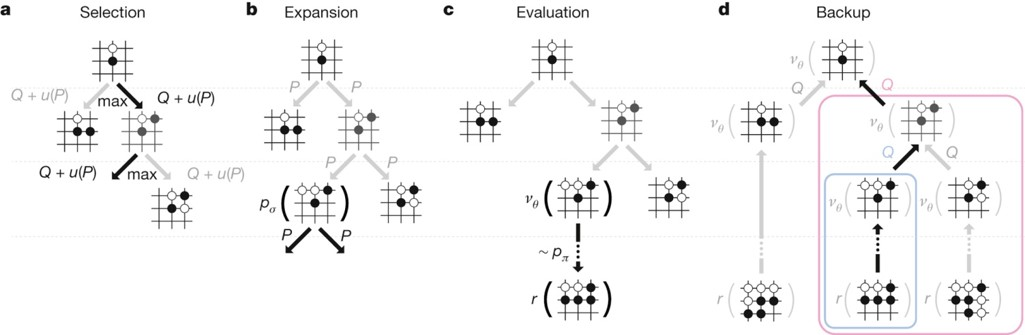
\includegraphics[width=\textwidth]{figures/alphago.jpg}
\caption{Monte Carlo tree search in AlphaGo 
Source:D Silver et al. Nature 529, 484–489 (2016) doi:10.1038/nature16961
 \label{figAlphaGO}}
\end{figure}

現今演算法的發展上已經逐漸地從利用人工設計的規則條件進展到讓機器自我建立規則的學習式機制,在各種領域如圖像辨識、資料探勘、自然語言處理、手寫文字識別、遊戲AI、機器人都有著蓬勃的發展,在這篇論文中預期以MCTS的角度切入,導入symbolic execution的路徑選擇演算法中,並比較其與傳統策略的效能差異。並希望在以MCTS為架構的演算法被建立後,在其之上加入機器學習的方法,如類神經網路、強化學習(Reinforcement learning)...,使得效能進一步增加,最後達到在漏洞挖掘上超越人類手工尋找的地步。





\chapter{Background}

在這個章節將簡要介紹symbolic execution與其遇到的問題,還有蒙地卡羅樹搜尋演算法的計算流程。

\section{Symbolic execution}

% 說明symbolic execution的流程和精神
在本篇論文中所提及的symbolic execution屬於Dynamic symbolic execution,首先由K. Sen\cite{sen2007concolic}提出,和基於其想法實作的程式DART\cite{godefroid2005dart}、CUTE\cite{sen2005cute},而其近年又分為兩種類型:需要程式原始碼的code-based symbolic execution如KLEE\cite{cadar2008klee},和不須程式碼而直接分析程式執行檔的binary-based symbolic execution如S2E\cite{chipounov2012s2e}、Mayhem\cite{cha2012mayhem}。symbolic execution engine在分析程式時會將其載入並先轉換為intermediate representation (IR),接著會將使用者輸入(例如標準輸入、檔案、命令列參數)標記為symbolic變數,接著模擬程式的執行過程,將執行過程中遇到的程式碼轉換為數學邏輯限制式的形式,當在模擬的過程中遇到分支條件時,便複製出一條新的路徑,分別追蹤該分支條件為真和為假時的情況;當模擬執行結束時,把先前蒐集的邏輯限制式利用solver求解(如:SMT\cite{vanegue2012smt}、Z3\cite{Z3}等等),以取得欲執行該路徑所需的實際輸入值;透過這個流程理論上我們可以追蹤所有的執行路徑,探索是否有不當的輸入值能觸發程式崩潰。

如下Figure \ref{figSE} 為一個簡單的binary-based symbolic execution執行時的狀況。它會依序讀入並根據指令進行相對應的模擬,位址4004f1將一個標記為symbolic variable的位址載入到暫存器eax中,則symbolic execution engine會在constraint table中標記eax為sym\_var1;4004f8將eax加3,symbolic execution engine則會在constraint table中記錄eax加3。當遇到分支跳轉指令時,如果無法決定該執行哪個分支,如Figure \ref{figSE} 中,eax的數值是一個symbolic variable,當使用者輸入不同數值,將導致不同的分支被執行,因此symbolic execution engine需要分別追蹤該分支為真和假時的狀態;由於每執行一條指令就返回顯得十分沒有效率,通常會讓symbolic execution engine遇到跳轉指令時,處理完狀態複製再返回,這樣的流程我們將其稱為一個步驟(step)。

\begin{figure}[htbp]
\center
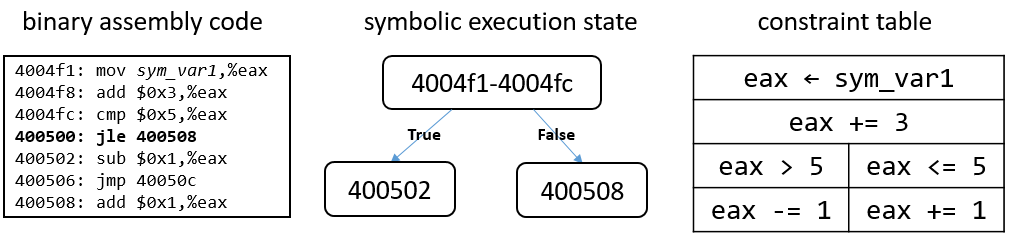
\includegraphics[width=\textwidth]{figures/SE.PNG}
\caption{symbolic execution流程 \label{figSE}}
\end{figure}

% 說明symbolic execution中的路徑探索問題
雖然symbolic execution理論上能夠探索所有執行路徑,但在探索的過程中會遭遇到上述的問題:當分支條件取決於symbolic variable時,很有可能兩邊的限制式都是可滿足的,這意謂著程式必須複製並分別維護兩條路徑,直到發現路徑無解為止,當越來越多路徑需要被追蹤,就產生了路徑爆炸問題(path explosion problem)。

\section{Monte Carlo tree search}

MCTS是一種啟發式搜尋演算法,近年來最廣為人知的應用是遊戲AI方面的演算法;Monte Carlo模擬是利用模擬和統計,得到一個近似解,在足夠大量的模擬下,理論上我們可以得到一個跟最佳解非常接近的答案。MCTS套用了這種模擬的方式,維護一棵樹(在遊戲AI中通常是一個遊戲盤面的狀態樹)並統計每個盤面的勝率,期望能只探索部分的樹,而非全部探索完的情況下,就能知道該盤面的勝率。

在\cite{browne2012surveyMCTS}中說明了MCTS演算法的基本流程,如Figure \ref{figMCTS}:

\begin{figure}[h]
\center
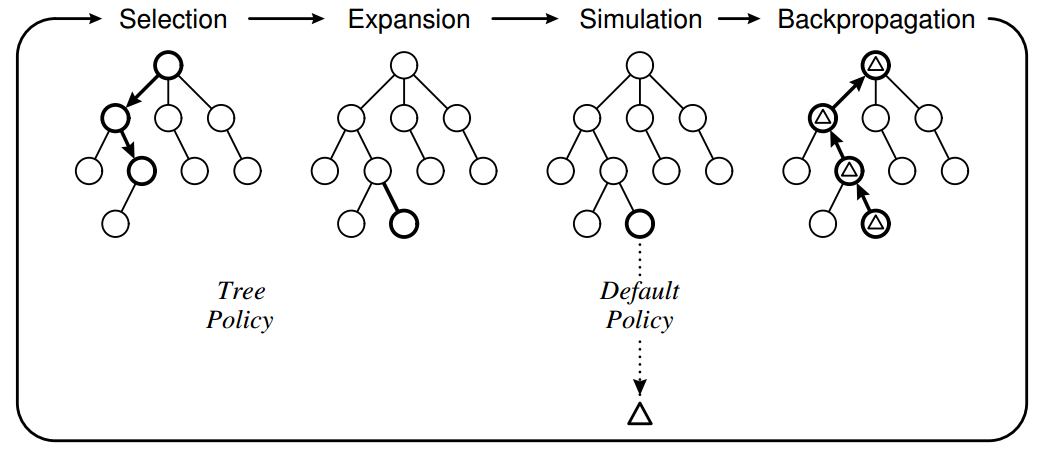
\includegraphics[width=\textwidth,height=\textheight,keepaspectratio]{figures/mcts2.PNG}
\caption{Monte Carlo Tree Search \label{figMCTS}}
\end{figure}

\begin{itemize}
\item \textbf{Selection} 根據設定的\textit{Tree Policy},從根節點開始遞迴性的決定一個目前最需要展開的節點,如Figure \ref{figMCTS}中的Selection部分,以粗框標記出的節點。可展開的節點在這裡定義為狀態尚未終止且有尚未訪問的子節點。
\item \textbf{Expansion} 在選擇的節點上,執行一個合法的動作來新增子節點,如Figure \ref{figMCTS}中的Expansion部分,在挑選的節點下新增一個節點。
\item \textbf{Simulation} 從這個新增的節點上使用\textit{Default Policy}來進行模擬執行,產生結果。
\item \textbf{Backpropagation} 模擬的結果會回饋到步驟1所選擇路過的那些節點上,更新他們的統計數據。
\end{itemize}

在這邊有兩個policy:\textit{Tree Policy}代表的是如何決定要選擇和新增節點的演算法。\textit{Default Policy}則是如何從該節點的狀態模擬對局直到獲得勝負結果。雖然這兩個Policy也可以簡單的使用隨機方式決定,但適當的演算法有助於強化MCTS的準確度,如\cite{Intro2MCTS}便指出,\textit{Tree Policy}可以使用upper confidence bound (UCB)演算法來取代隨機挑選,如果我們把盤面的位置當成吃角子老虎機,視為multi-armed bandit problem來處理的話,會比原本的隨機選擇好;另外他也指出模擬時除了用這些簡單的方法,也可以使用更耗費資源的啟發式邏輯和評價方式,在對於higher branching factor的遊戲會有較好的效果。

\chapter{Method}

\section{Motivation example}

在不同策略下,樹的走訪順序如Firuge \ref{figST}所示,假設固定先選擇的都是左子樹,DFS會優先選擇最深的節點來走訪,而BFS選擇最淺的節點,這兩個策略都有一樣的問題:順序是固定的,如DFS很可能因為左子樹太過龐大,但較高效益的節點在右子樹,而浪費很多時間在走訪較低效益的節點;又如BFS,很可能較高效益的節點要往深處搜尋,但走訪深度較淺的節點就已經花費不少時間。它們共同的問題就是走訪到節點5、6的順序都一樣是在最後面。而MCTS的走訪順序是不固定的,它會動態的選擇一個被認為是目前最應該走訪的節點來進行計算。

\begin{figure}[htbp]
\center
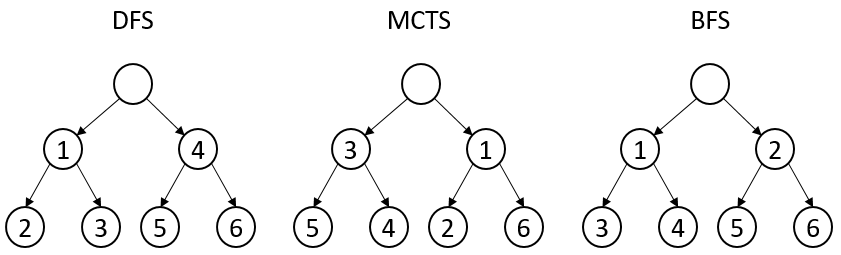
\includegraphics[width=\textwidth]{figures/strategy.PNG}
\caption{不同策略的樹走訪順序 \label{figST}}
\end{figure}

Figure \ref{figTREE}為範例程式碼Algorithm 1在symbolic execution計算過程中所建立的狀態樹,每個節點都代表著一個狀態,包含了程式的暫存器和記憶體內容,symbolic variables的constraint等等。root節點代表剛進入該段程式的狀態,而其左子節點則是執行完第1行時的狀態,我們以數字1來標記該節點目前執行的位址,沒有標記數字的節點則是代表程式結束,其他節點也以此類推。

\begin{figure}[htbp]
\center
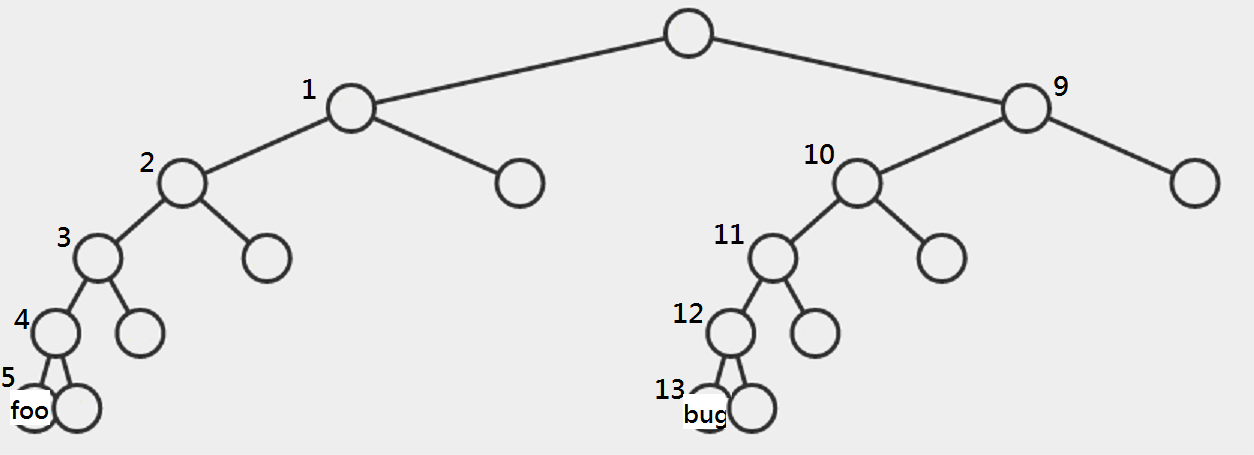
\includegraphics[width=\textwidth]{figures/tree.png}
\caption{Tree of the example code \label{figTREE}}
\end{figure}

從Figure \ref{figTREE}這棵樹中我們可以發現,當使用DFS來進行搜索時,程式需要先走訪完整個左子樹才有可能執行到bug函式,更壞的情況是有可能左子樹大到無法走完,程式被困在其中進行無效的運算;而如果使用BFS來搜索時,雖然最後foo函式和bug函式會在差不多的時間點被執行到,但很有可能因為在過程中已經發現太多節點,而造成記憶體空間不足的問題;所以我們希望採用一個策略,是程式能動態決定該選擇哪個節點來往下走訪的。

\newpage

\begin{algorithm}[htbp]
  \caption{Example Code}
  \begin{algorithmic}[1]
    \If{$w>5$}
    	\If{$x>10$}
        	\If{$y>20$}
            	\If{$z>30$}
                	\State foo()
                \EndIf
            \EndIf
        \EndIf
    \Else
        \If{$x>10$}
        	\If{$y>20$}
            	\If{$z>30$}
                	\State bug()
                \EndIf
            \EndIf
        \EndIf
    \EndIf
  \end{algorithmic}
\end{algorithm}

對symbolic execution而言,不管採用哪種搜尋策略,我們的目標都是:如何達到更高的程式碼覆蓋率,以盡可能的測試出不同執行狀態時,程式是否會發生錯誤或崩潰。我們希望採用MCTS演算法來搜索時,能比傳統的搜尋方法能在同樣的資源限制下(如時間限制、記憶體限制)走訪更多的程式碼。

\section{proposed algorithm}

\begin{algorithm}[htbp]
  \caption{applying MCTS algorithm to symbolic execution}
  \begin{algorithmic}[1]
  	\Function{Search}{$p_r$}
    \State set $p_r$ as root of Tree $T$
    \State $B \leftarrow \emptyset$
    \While {within computational budget}
      \State $p$ $\leftarrow$ TreePolicy($T$)
      \State $B \leftarrow B \bigcup p$
      \State $S$ $\leftarrow$ step($p$)
      \For{each path $p_c \in S$}
      	\State $V \leftarrow$ DefaultPolicy($p_c$)
        \State $Q(p_c) \leftarrow \alpha \frac{|V-B|}{N} + \beta|p_c|$
        \State add a new child $p_c$ to $p$
      \EndFor
      \State BackPropagation($p$)
    \EndWhile
    \EndFunction
  \end{algorithmic}
\end{algorithm}

Algorithm 2 為我們設計的演算法主體。$p_r$為現在要搜尋的路徑,首先將$p_r$設為樹$T$的root,以記錄路徑間的關係,並以集合$B$來計算路徑走訪的數量。在第5行我們會先利用\textit{Tree Policy}從樹$T$中挑選一個應該計算的路徑$p$,並將$p$加進集合$B$中(路徑$p$事實上可以被視為是數個走訪過的位址集合),接著將$p$遞交給symbolic execution engine進行計算,symbolic execution engine會將這條路徑step(往下執行若干條指令,直到遇見分支跳轉指令才停止);step後可能產生數條路徑,我們以集合$S$來表示,$S$中的路徑代表$p$ step後可能的狀態,如執行if時或執行else時的狀態,遇到switch case時執行不同case的狀態;在第8行對$S$中的每條路徑$p_c$我們都會利用\textit{Default Policy}來模擬其未來可能的走向,並評估此路徑的價值$Q(p_c)$,將$p_c$標記為$p$的child;最後在第13行整理先前第8-12行的資訊並記錄起來。

在第10行為我們計算路徑價值的公式,此公式分為兩個部分,其中$\alpha$、$\beta$和$N$為可以人為控制的參數。$\frac{|V-B|}{N}$中的$V$為路徑$p_c$經由\textit{Default Policy}計算後得出未來可能會執行的位址集合,和集合$B$取差集後計算其數量,除以$N$(\textit{Default Policy}模擬的次數)就是路徑$p_c$增加程式執行區塊覆蓋率的期望值;而$|p_c|$為$p_c$執行過的程式碼區塊數量,這個參數是為了在所有路徑的覆蓋率期望值都非常低的時候,能優先選擇較深的路徑避免進行無謂的探索。$\alpha$和$\beta$是這兩個數值的權重。計算$Q$時的$\alpha$主要控制的是增加覆蓋率的期望值,由於路徑的模擬是根據Control flow graph(CFG)來猜測,如果產生的CFG不正確(不同的實作方式可能產生不同結果)或程式的實際執行狀況和模擬的結果有落差,期望值就會變得不準確,相對的對於簡單的小程式,模擬的準確度有可能是較高的,因此適當的調整$\alpha$可以修正模擬的數據;而$\beta$是為了因應遇到大量迴圈或strcmp這類函式的措施,由於進入迴圈容易產生大量的分枝,會讓path數量一下子成長很多,\textit{Tree Policy}在選擇時也容易被混淆,我們透過計算該path已經執行過的程式碼區塊數量,讓演算法在挑選時偏好已經執行比較多區塊數量的路徑。

Algorithm 3是Algorithm 2中所提及的函式實作部分。\textit{Tree Policy}用來挑選應該被計算的路徑,而價值計算事實上是由$BestChild$決定,其中的一個參數$C$,其影響的是MCTS中最大的特徵:expolitation和exploration,也就是程式該往較深的點進行計算,還是選擇較少被計算過的點,不過這個數值在branching factor高時較有效,而我們產生出的path常常只有1至2個,所以這個參數的影響並不大,唯一會影響的是當某個節點尚未被計算過任何一次的時候,$N(p_c)$為0,根號內的數值會是無限大,程式就一定會選擇該節點來進行計算。\textit{Default Policy}的參數$N,M$,$N$是要進行幾次模擬,而$M$是避免程式進入無窮迴圈,當到達一定數字時會強制中斷模擬,對於較小的程式可以選擇較小的數字,而較複雜的程式可以選擇比較大的數字來增加其準確性,但也相對的花費更多時間。$BackPropagation$會更新兩項數值,$N(v)$為$v$被訪問的次數,對於價值$Q(v)$則以$v$的子節點們的平均來替代。

\begin{algorithm}[H]
  \caption{Policies for our algorithm}
  \begin{algorithmic}[]
    \Function{TreePolicy}{$T$}
    	\State $n \leftarrow$ root of $T$
        \While {$n$ is not terminated}
        	\If{$n$ is expandable}
            	\State \Return {$n$}
            \Else
            	\State $n \leftarrow BestChild(n,C)$
            \EndIf
        \EndWhile
    \EndFunction
    \item[]
	\Function{DefaultPolicy}{$p$}
    	\State $V \leftarrow \emptyset$
        \For{$i=1$; $i<N$; $i++$}
          \State $v \leftarrow$ find vertex at CFG($p$'s addr)
          \For{$j=1$; ($j<M$)and($v$ has any edge); $j++$}
              \State add $v$ to $V$
              \State $v \leftarrow$ random pick a vertex which $v$ directed to
          \EndFor
        \EndFor
        \State \Return $V$
    \EndFunction
    \item[]
    \Function{BestChild}{$p,C$}
    	\State $Q_{max} \leftarrow \operatorname*{arg\,max}_{p_c \in p} Q(p_c)$
    	\State \[ \Return \argmax_{p_c \in p} \frac{Q(p_c)}{Q_{max}}+C\sqrt[]{\frac{2\ln N(p)}{N(p_c)}} \]
    \EndFunction
    \item[]
    \Function{BackPropagation}{$v$}
    \While{$v$ is not null}
    	\State N($v$) += 1
		\State Q($v$) $\leftarrow$ average of Q($v$'s children)
    \State $v \leftarrow$ parent of $v$
    \EndWhile
    \EndFunction
  \end{algorithmic}
\end{algorithm}

\section{algorithm explanation}

如下Figure \ref{figStep} 為MCTS簡要的執行過程示意圖。在Step 1設定根節點後,由於沒有任何子節點,我們在Selection階段便直接選擇根節點,進行Expansion後新增兩個子節點,其價值經Simulation計算後分別為60和80。Step 2從根節點找到兩個子節點,在這邊選擇價值為80的子節點進行Expansion,得到兩個子節點並計算出其價值為50和52,獲得子節點的估計價值後,便可以作為Backpropagation使用,節點1的價值將改由其子節點價值的平均來取代,如這邊即從80變為51。Step 3因為在Step 2時修正了節點1的價值,在Selection階段便會轉而選擇節點2,經過Expansion和Simulation後同樣利用子節點來修正節點2的價值,不斷的重複這個步驟來挑選最應該被計算的節點。

\begin{figure}[htbp]
\center
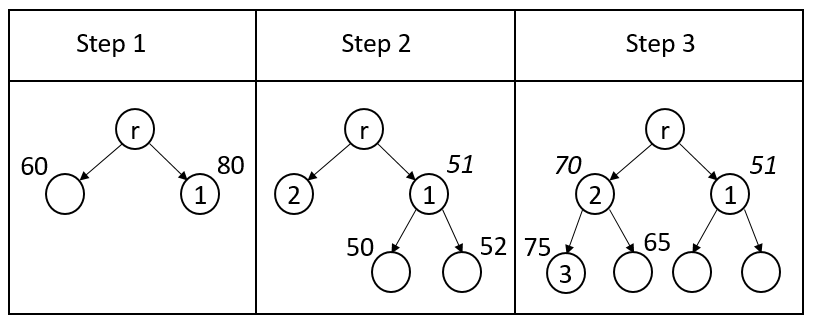
\includegraphics[width=\textwidth]{figures/step.PNG}
\caption{MCTS執行過程 \label{figStep}}
\end{figure}

\chapter{Implementation}

\section{Angr's architecture}

Angr\cite{angr} 是一個支援多種架構的程式分析平台,主要以python撰寫,能夠執行如dynamic symbolic execution和多種靜態分析方法。這個平台可以自動替使用者完成一些工作,如:讀取並載入程式binary到分析平台中、將程式binary轉換成intermediate representation (IR),程式靜態分析,如:相依性分析、control flow graph、data flow graph。Angr主要擁有以下幾個元件:binary loader可以載入不同平台的程式、Intermediate representation讓不同格式的程式都能使用同一套演算法或工具、Solver Engine以計算出symbolic execution中的變數值、Program states以模擬機器的狀態,如暫存器目前的值、Program paths以記錄程式執行的路徑作為分析用、symbolic execution和program analysis。

要使用Angr進行程式分析必須自行撰寫python script來呼叫相關功能,如Figure \ref{figScript}為使用Angr執行symbolic execution的範例script;與作業系統執行process的過程類似,首先執行Line 22,必須找到程式的binary位置並傳給Angr進行初始化,由於程式大多會連結多個函式庫,如果將其視為程式的一部份一同載入會使得載入時間變得很長,因此在Line 14選擇關閉一同載入的功能,直到程式執行到該地方了再去載入函式庫;接著必須使用Angr內的solver engine:claripy來設定symbolic variables,以程式gif2png為例,執行的時候只需要給他兩個命令列選項,而第二個選項為圖片位置,所以我們將第一個選項設為symbolic variable,使用claripy的BVS (symbolic bitvector)物件,並給它一個名稱和初始值;再來的Line 16則是將設定好的程式啟動並執行到某個狀態,當程式要執行時除了讀取程式binary外還要設定它的記憶體區段、初始化數值、環境變數等等資訊,而我們所寫的entry是指這些資訊都設定完成時,程式剛要從程式進入點開始執行的狀態;另外我們還可以給它一些其它設定,如命令列參數傳入了剛剛宣告的symbolic variable,還有檔案的名稱,也可以設定執行時要開啟或關閉哪些選項,在這邊關閉了LAZY\_SOLVES功能,讓Angr會自動移除unsatisfiable的路徑;這些前置工作都完成後才獲得預備要進行symbolic execution的初始化狀態,接著在Line 18使用Angr的path\_group功能來代替我們管理symbolic execution的繁瑣設定;path\_group代表的是一群path的集合,當symbolic execution在執行時會不斷的增長出新的path,而path\_group可以將path進行分類,如:errored、unconstrainted、pruned、deadended、unsatisfiable等等,此外還能過濾、合併、複製路徑,或是設定symbolic execution要停止的條件,是一個功能相當強大的class。最後利用path\_group的run function就可以幫我們執行symbolic execution。

\begin{figure}[htbp]
\center
\includegraphics[width=\textwidth]{figures/script.png}
\caption{Example script to run symbolic execution in Angr \label{figScript}}
\end{figure}

%%%%%%%%%%%%%%%%%%%%%%%%%%%%%%%%%
\section{Exploration techniques}

前一節提到了path\_group,在它內部也實作了一套方法可以讓使用者撰寫不同的exploration technique來應用到symbolic execution上,在提到exploration technique前必須先提及的是path\_group內執行symbolic execution的方法,我們呼叫的方法是run,其內部呼叫了step使其進行無數次迴圈,如Figure \ref{figAngrStep}為部分原始碼,run會將n設為一個極大值;而step真正呼叫的是\_one\_step function,執行後檢查是否還需要繼續執行,不斷進行迴圈。

\begin{figure}[htbp]
\center
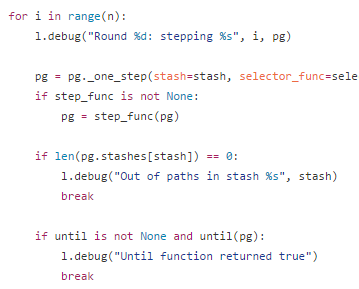
\includegraphics[]{figures/angrStep.png}
\caption{partial code of step in Angr \label{figAngrStep}}
\end{figure}

\_one\_step function內才是真正會呼叫exploration techniques提供的方法之處,在啟用每個exploration technique時,Angr會將它們提供的四種方法:step、step\_path、filter、complete給加入hook function內,如Figure \ref{figAngrOneStep}中的變數\_hook\_step為一個陣列,裡面存放不同exploration techniques提供的step function,首先它會將一個step function取出,並執行該step function,而exploration technique提供的step function需要再呼叫一次step,這時如果還有其他hook的step就會取出來繼續執行,否則就會執行原生的step function,如Figure \ref{figExptech}為Exploration technique DFS的step function實作,Line 16先呼叫step後,才執行其對路徑的重新選擇。我們可以將exploration technique的step分為兩個部分,一為step前處理,一為step後處理,論文中的MCTS演算法實作完全是環繞於這兩個區塊而成。

\begin{figure}[htbp]
\center
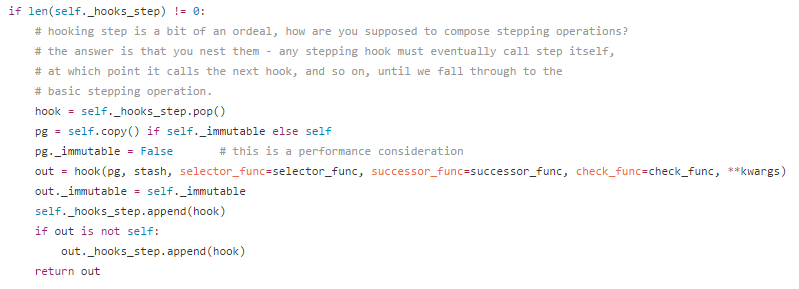
\includegraphics[]{figures/oneStep.png}
\caption{partial code of one step in Angr \label{figAngrOneStep}}
\end{figure}

\begin{figure}[htbp]
\center
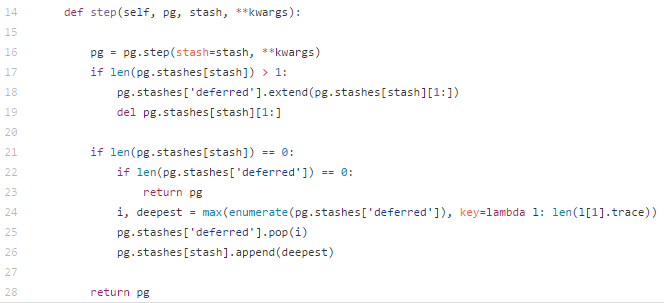
\includegraphics[]{figures/exptech.png}
\caption{partial code of exploration technique(DFS) in Angr \label{figExptech}}
\end{figure}

%%%%%%%%%%%%%%%%%%%%%%%%%%%%%%%%%
\section{Applied MCTS into Angr}

Figure \ref{figPreStep}是MCTS在step前所作的處理,對於接下來要用symbolic execution計算的路徑,會先取出該路徑的歷史路徑位址集合,並更新到目前總共執行過的位址集合中,這個集合在之後會用來判斷路徑是不是有可能增加覆蓋率,由於每次都只會有一條路徑在stash中準備要進行計算,所以我們只取出一條即可。

\begin{figure}[htbp]
\center
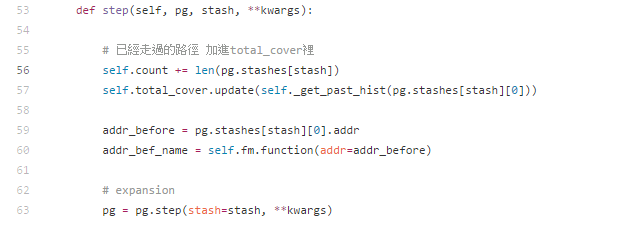
\includegraphics[]{figures/preStep.png}
\caption{MCTS of pre step in Angr \label{figPreStep}}
\end{figure}

呼叫完原本的step function後,就等同於演算法中的Expansion階段已經完成了,之後會進行MCTS的計算處理,如Figure \ref{figPostStep},現在stash中的路徑都是剛剛進去計算的路徑的子節點,我們會將每一條都取出來,並進行Simulation,得到平均可增加覆蓋率後,將子節點增加到tree中。之後呼叫tree的refresh\_tree function,也就是演算法的backpropagation階段。最後才執行Selection,雖然是為了配合Angr的設計,但在演算法上步驟的調整並不影響計算,在這個階段會呼叫tree的select\_node function幫我們找出最好的那個節點。

\begin{figure}[htbp]
\center
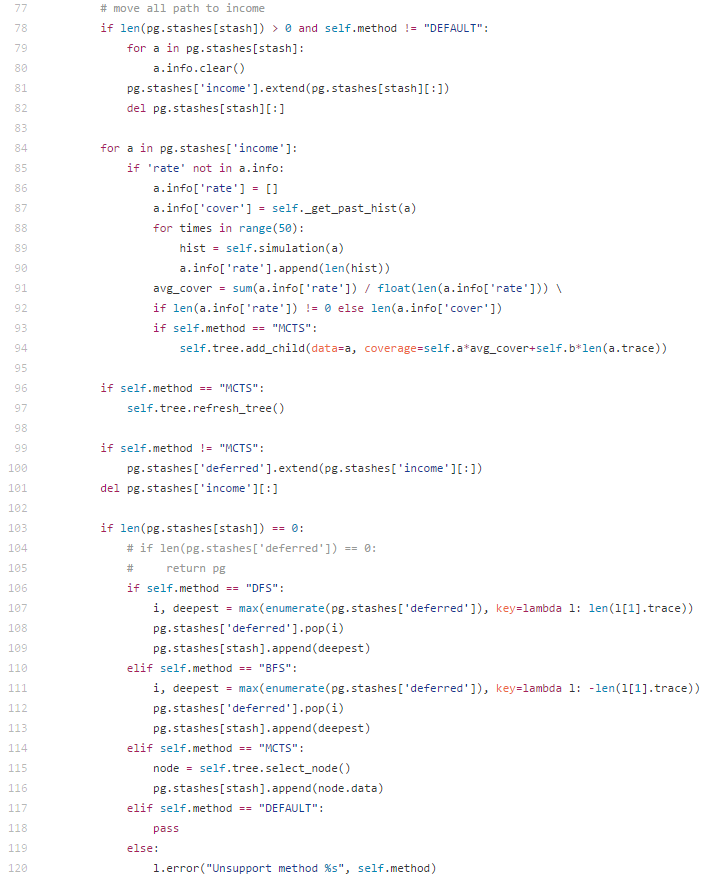
\includegraphics[]{figures/postStep.png}
\caption{MCTS of post step in Angr \label{figPostStep}}
\end{figure}



\chapter{Result and Evaluation}

\section{Environment}

我們將本篇論文提出的演算法實作於Angr (一個開源的python符號執行框架) \cite{angr}上,並在Ubuntu 16.04作業系統環境進行實驗,受測程式如Table \ref{binarys}。硬體環境使用的是Intel i7-2600k處理器以及24 GB記憶體。主要比較的目標是演算法經由symbolic execution所執行過的程式碼區塊數量:程式碼區塊指的是一段程式碼中間沒有任何的跳轉指令,而以跳轉指令為結尾,也就是說程式碼區塊執行直到最後一個指令時才會跳轉到其他區塊,每個區塊都不會發生與其他區塊有所重疊或覆蓋的情形;我們以程式碼區塊的第一條指令位址為其開始位址並作為判斷是否重複的標準,對重複執行過的區塊我們只會計算一次而不是會重複計算多次。在前章所提及的演算法參數,由於參數調校並非本篇論文的重點,因此在所有實驗中都固定使用同一組參數來進行。

\newcommand{\ra}[1]{\renewcommand{\arraystretch}{#1}}
\begin{table*}[htbp]\centering
\caption{Target Program's name and version}
\label{binarys}
\begin{tabular}{@{}ll@{}}\toprule
program name & version \\ \midrule
cp           & 8.25    \\ 
echo         & 8.25    \\ 
hostname     & 3.16    \\ 
ls           & 8.25    \\ 
mkdir        & 8.25    \\ 
ps           & 3.3.10  \\ 
readelf      & 2.26.1  \\ 
touch        & 8.25    \\ 
cpp-markdown & 1.00    \\ 
gif2png      & 2.5.8   \\ \bottomrule
\end{tabular}
\end{table*}

\section{演算法與其他方法的比較}

% 3k step, BFS, DFS, MCTS
為了比較不同方法間的效率好壞,我們給定一個資源限制:程式最多只能使用symbolic execution engine來step 3000次,對時間和記憶體用量皆未限制。Table \ref{testMethod}是在此限制下MCTS和DFS、BFS比較的結果。其中數量為前一節所述的程式碼區塊數量,時間為該次實驗的執行時間(秒),效率則是區塊數量除以時間後得到每秒會增加的平均值。

\begin{table}[htbp]
\ra{1.3}
\centering
\caption{Comparison of the efficiency with different strategies}
\label{testMethod}
\begin{tabular}{@{}llllllllllll@{}} \toprule
             & \multicolumn{3}{c}{MCTS} & \phantom{abc} & \multicolumn{3}{c}{DFS} & \phantom{abc} & \multicolumn{3}{c}{BFS} \\ \cmidrule{2-4} \cmidrule{6-8} \cmidrule{10-12}
program      & \#   & time(s)   & eft   & & \#   & time(s)   & eft   & & \#    & time(s)   & eft      \\ \midrule
cpp-markdown & 566    & 272.07 & 2.08 & & 529    & 306.27& 1.73  & & 478     & 318.16 & 1.50   \\
cp           & 388    & 3732.45& 0.10 & & 218    &2340.34& 0.09  & & 174     & 326.38 & 0.53   \\
echo         &  84    & 164.90 & 0.51 & &  76    & 283.49& 0.27  & &  83     & 126.61 & 0.66   \\
gif2png      & 105    & 192.66 & 0.55 & &  64    &2115.42& 0.03  & &  59     & 680.98 & 0.09   \\ 
hostname     & 175    & 277.80 & 0.63 & &  62    & 147.08& 0.42  & &  61     & 309.11 & 0.20   \\
ls           & 393    & 715.55 & 0.55 & & 189    &1053.82& 0.18  & & 152     &3057.35 & 0.05   \\
mkdir        & 320    & 275.96 & 1.16 & &  82    & 142.86& 0.57  & & 119     & 198.10 & 0.60   \\
ps           &  99    & 682.35 & 0.15 & & 185    & 176.52& 1.05  & & 109     &1083.84 & 0.10   \\
readelf      & 288    & 870.36 & 0.33 & & 393    & 913.68& 0.43  & & 156     &1179.49 & 0.13   \\
touch        & 302    & 331.78 & 0.91 & & 213    &1665.38& 0.13  & & 124     & 194.40 & 0.64   \\ \hline
avg.         & 272    & 751.59 & 0.70 & & 201.1  & 914.49& 0.49  & & 151.5   & 747.44 & 0.45   \\
SD           & 148.51 &1020.75 & 0.55 & & 145.99 & 809.66& 0.50  & & 114.97  & 847.74 & 0.42   \\ \bottomrule
% sum          & 2720   & 7515.88& 6.96 & & 2011   &9144.86& 4.90  & & 1515    &7474.42 & 4.50   \\ \bottomrule
\end{tabular}
\end{table}

為了方便比較我們將數值繪製成折線圖,如Figure \ref{figCoverageSmall},可以看到MCTS在大部分的實驗都是勝出的,只有兩隻程式的數值較差。接著比較其效率,結果如Figure \ref{figEffSmall},除了原本的兩隻程式外,還有兩隻程式遜於BFS,但仍贏過DFS。雖然各有勝負,但從數據的平均值來看,MCTS的效能是比較好的,而標準差也可以看出對實驗結果的不確定性,MCTS相對於其他兩個方法並沒有極大的差異。

\begin{figure}[htbp]
\center
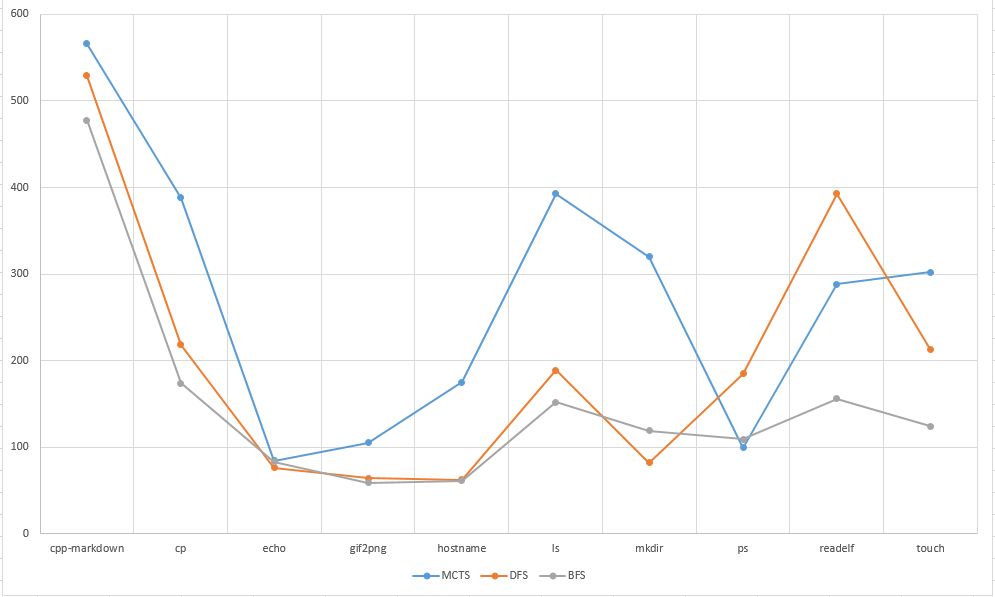
\includegraphics[width=\textwidth]{figures/small_block.png}
\caption{block coverage in small test \label{figCoverageSmall}}
\end{figure}

\begin{figure}[htbp]
\center
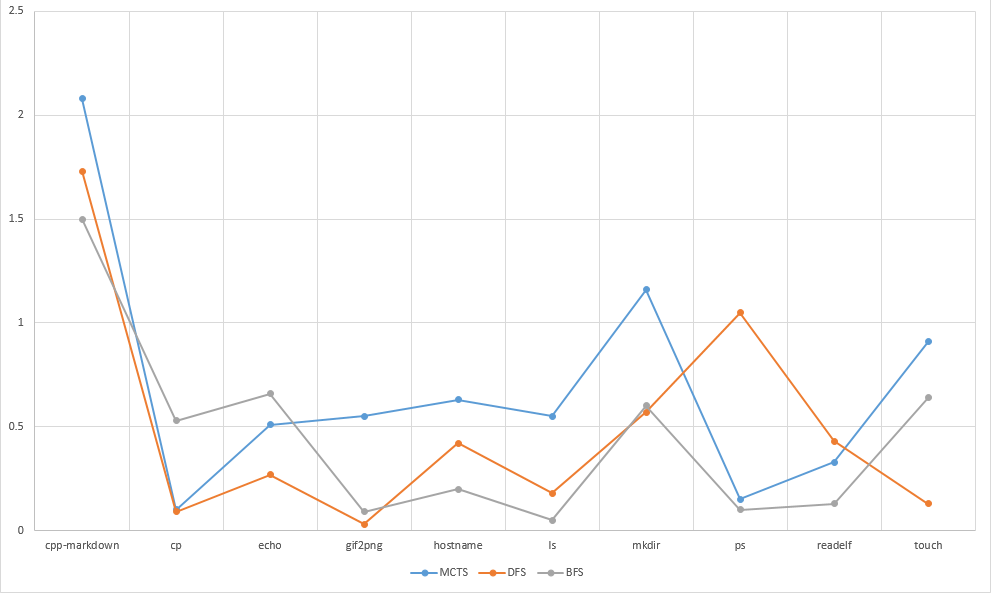
\includegraphics[width=\textwidth]{figures/small_eff.png}
\caption{efficienct in small test \label{figEffSmall}}
\end{figure}

\section{MCTS的評估函式效能測量}

在演算法中的Selection階段會遞迴性的選擇最好的子節點直到發現一個可展開的節點,而Simulation階段也會根據先前展開的節點來模擬評估其價值,這兩個階段在演算法中位居引導演算法的重要角色,因此我們想要知道如果沒有這兩個階段之下,演算法的效能如何,下面比較的對象是將Selection從選擇BestChild改為隨機選擇一個子節點,結果如Table \ref{testRandomSeletion}所示,結果只有程式echo和ps略輸於Random,但差距非常的小,只有3.5\%,單從區塊涵蓋數量來看,平均有35\%的成長,而Random甚至略遜於DFS的平均值,除上執行時間後,效率更加糟糕,這有可能是因為symbolic execution本身的優化技巧在隨機選擇後沒有辦法發揮效果,以至於平均執行時間增加到2.7倍。

\begin{table}[htbp]
\ra{1.3}
\centering
\caption{Comparison of the efficiency with random selection}
\label{testRandomSeletion}
\begin{tabular}{@{}lllllllll@{}} \toprule
             & \multicolumn{3}{c}{MCTS} & \phantom{abc} & \multicolumn{3}{c}{Random} \\ \cmidrule{2-4} \cmidrule{6-8}
program      & \#   & time(s)   & eft   & & \#   & time(s) & eft  \\ \midrule
cpp-markdown & 566    & 272.07 & 2.08 & & 479    &2013.28& 0.24     \\
cp           & 388    & 3732.45& 0.10 & & 265    &2038.27& 0.13     \\
echo         &  84    & 164.90 & 0.51 & &  87    & 575.15& 0.15     \\
gif2png      & 105    & 192.66 & 0.55 & & 101    &1116.26& 0.09     \\ 
hostname     & 175    & 277.80 & 0.63 & &  94    & 826.82& 0.11     \\
ls           & 393    & 715.55 & 0.55 & & 168    &3374.23& 0.05     \\
mkdir        & 320    & 275.96 & 1.16 & & 187    &1154.84& 0.16     \\
ps           &  99    & 682.35 & 0.15 & & 103    &1631   & 0.06     \\
readelf      & 288    & 870.36 & 0.33 & & 263    &6599.76& 0.03     \\
touch        & 302    & 331.78 & 0.91 & & 246    &1025.58& 0.24     \\ \hline
avg.         & 272    & 751.59 & 0.70 & & 199.3  &2035.52& 0.13     \\
SD           & 148.51 &1020.75 & 0.55 & & 115.13 &1703.61& 0.07     \\ \bottomrule
\end{tabular}
\end{table}

\section{長時間執行的效率比較}

% 24hr + 20G limit (usually 50k~100k step), BFS, DFS, MCTS
經小規模實驗得到MCTS較佳的結果後,我們用較大規模的方法來實驗,前項實驗的執行時間大約為13分鐘上下,且記憶體用量幾乎不會超過2 GB;因此在這個實驗我們改以24小時的時間限制和20 GB的記憶體用量限制,而不限制其在symbolic execution engine的step次數,來觀察在有限的記憶體用量下,我們的方法相較於傳統的方法能有多少幅度的效率成長。

%%%%%%%%%%%%%%%%%
% cpp-markdown
%%%%%%%%%%%%%%%%%
\begin{figure}[htbp]
\center
\begin{tikzpicture}
\begin{axis}[
    title={cpp-markdown},
    xlabel={step times},
    ylabel={number of basic blocks coverage},
    xmin=0, xmax=100000,
    ymin=0, ymax=800,
    width=\textwidth,
    height=\textheight/2-3cm,
    xtick={0,100,500,1000,2000,5000,20000,100000},
    ytick={0,100,200,300,400,500,600,700,800},
    legend pos=north west,
    ymajorgrids=true,
    grid style=dashed,
    xmode=log,
    log ticks with fixed point,
]
 
\addplot[
    color=blue,
    mark=square,
    ]
    coordinates {
    (100,47)(500,199)(1000,349)(2000,477)(5000,541)(10000,559)(20000,593)(100000,606)
    };
    \addlegendentry{MCTS}

\addplot[
    color=red,
    mark=triangle,
    ]
    coordinates {
    (100,47)(500,205)(1000,376)(2000,497)(5000,572)(10000,579)(20000,579)(100000,588)
    };
    \addlegendentry{DFS}

\addplot[
    color=green,
    mark=star,
    ]
    coordinates {
    (100,47)(500,196)(1000,385)(2000,459)(5000,519)(10000,560)(20000,629)(100000,661)
    };
    \addlegendentry{BFS}

\end{axis}
\end{tikzpicture}
\caption{large test for cpp-markdown \label{test_cpp-markdown}}
\end{figure}

%%%%%%%%%%%%%%%%%
% cp
%%%%%%%%%%%%%%%%%
\begin{figure}[htbp]
\center
\begin{tikzpicture}
\begin{axis}[
    title={cp},
    xlabel={step times},
    ylabel={number of basic blocks coverage},
    xmin=0, xmax=20000,
    ymin=0, ymax=700,
    width=\textwidth,
    height=\textheight/2-3cm,
    xtick={0,100,500,1000,2000,5000,20000},
    ytick={0,100,200,300,400,500,600,700},
    legend pos=north west,
    ymajorgrids=true,
    grid style=dashed,
    xmode=log,
    log ticks with fixed point,
]
 
\addplot[
    color=blue,
    mark=square,
    ]
    coordinates {
    (100,38)(500,119)(1000,202)(2000,331)(5000,462)(10000,573)(17000,581)
    };
    \addlegendentry{MCTS}

\addplot[
    color=red,
    mark=triangle,
    ]
    coordinates {
    (100,47)(500,164)(1000,178)(2000,186)(5000,222)(10000,222)(20000,222)
    };
    \addlegendentry{DFS}

\addplot[
    color=green,
    mark=star,
    ]
    coordinates {
    (100,24)(500,50)(1000,92)(2000,126)(5000,196)(10000,215)(20000,226)
    };
    \addlegendentry{BFS}

\end{axis}
\end{tikzpicture}
\caption{large test for cp \label{test_cp}}
\end{figure}

%%%%%%%%%%%%%%%%%
% echo
%%%%%%%%%%%%%%%%%
\begin{figure}[htbp]
\center
\begin{tikzpicture}
\begin{axis}[
    title={echo},
    xlabel={step times},
    ylabel={number of basic blocks coverage},
    xmin=0, xmax=20000,
    ymin=0, ymax=150,
    width=\textwidth,
    height=\textheight/2-3cm,
    xtick={0,100,500,1000,2000,5000,20000},
    ytick={0,20,40,60,80,100,120,140},
    legend pos=north west,
    ymajorgrids=true,
    grid style=dashed,
    xmode=log,
    log ticks with fixed point,
]
 
\addplot[
    color=blue,
    mark=square,
    ]
    coordinates {
    (100,37)(500,67)(1000,71)(2000,79)(5000,92)(10000,93)(20000,102)
    };
    \addlegendentry{MCTS}

\addplot[
    color=red,
    mark=triangle,
    ]
    coordinates {
    (100,34)(500,52)(1000,57)(2000,71)(5000,84)(10000,87)(20000,87)
    };
    \addlegendentry{DFS}

\addplot[
    color=green,
    mark=star,
    ]
    coordinates {
    (100,27)(500,43)(1000,57)(2000,77)(5000,105)(10000,118)(20000,129)
    };
    \addlegendentry{BFS}

\end{axis}
\end{tikzpicture}
\caption{large test for echo \label{test_echo}}
\end{figure}

%%%%%%%%%%%%%%%%%
% gif2png
%%%%%%%%%%%%%%%%%
\begin{figure}[htbp]
\center
\begin{tikzpicture}
\begin{axis}[
    title={gif2png},
    xlabel={step times},
    ylabel={number of basic blocks coverage},
    xmin=0, xmax=20000,
    ymin=0, ymax=150,
    width=\textwidth,
    height=\textheight/2-3cm,
    xtick={0,100,500,1000,2000,5000,20000},
    ytick={0,20,40,60,80,100,120,140},
    legend pos=north west,
    ymajorgrids=true,
    grid style=dashed,
    xmode=log,
    log ticks with fixed point,
]
 
\addplot[
    color=blue,
    mark=square,
    ]
    coordinates {
    (100,26)(500,70)(1000,96)(2000,107)(5000,107)(10000,107)(20000,107)
    };
    \addlegendentry{MCTS}

\addplot[
    color=red,
    mark=triangle,
    ]
    coordinates {
    (100,14)(500,34)(1000,64)(2000,64)(5000,64)(10000,64)(20000,64)
    };
    \addlegendentry{DFS}

\addplot[
    color=green,
    mark=star,
    ]
    coordinates {
    (100,23)(500,49)(1000,53)(2000,58)(5000,61)(10000,63)(20000,73)
    };
    \addlegendentry{BFS}

\end{axis}
\end{tikzpicture}
\caption{large test for gif2png \label{test_gif2png}}
\end{figure}

%%%%%%%%%%%%%%%%%
% hostname
%%%%%%%%%%%%%%%%%
\begin{figure}[htbp]
\center
\begin{tikzpicture}
\begin{axis}[
    title={hostname},
    xlabel={step times},
    ylabel={number of basic blocks coverage},
    xmin=0, xmax=20000,
    ymin=0, ymax=200,
    width=\textwidth,
    height=\textheight/2-3cm,
    xtick={0,100,500,1000,2000,5000,20000},
    ytick={0,40,80,120,160,200},
    legend pos=north west,
    ymajorgrids=true,
    grid style=dashed,
    xmode=log,
    log ticks with fixed point,
]
 
\addplot[
    color=blue,
    mark=square,
    ]
    coordinates {
    (100,25)(500,95)(1000,128)(2000,146)(5000,184)(10000,184)(20000,184)
    };
    \addlegendentry{MCTS}

\addplot[
    color=red,
    mark=triangle,
    ]
    coordinates {
    (100,35)(500,61)(1000,61)(2000,61)(5000,61)(10000,61)(20000,61)
    };
    \addlegendentry{DFS}

\addplot[
    color=green,
    mark=star,
    ]
    coordinates {
    (100,19)(500,57)(1000,60)(2000,61)(5000,63)(10000,64)(20000,65)
    };
    \addlegendentry{BFS}

\end{axis}
\end{tikzpicture}
\caption{large test for hostname \label{test_hostname}}
\end{figure}


%%%%%%%%%%%%%%%%%
% ls
%%%%%%%%%%%%%%%%%
\begin{figure}[htbp]
\center
\begin{tikzpicture}
\begin{axis}[
    title={ls},
    xlabel={step times},
    ylabel={number of basic blocks coverage},
    xmin=0, xmax=20000,
    ymin=0, ymax=700,
    width=\textwidth,
    height=\textheight/2-3cm,
    xtick={0,100,500,1000,2000,5000,20000},
    ytick={0,100,200,300,400,500,600,700},
    legend pos=north west,
    ymajorgrids=true,
    grid style=dashed,
    xmode=log,
    log ticks with fixed point,
]
 
\addplot[
    color=blue,
    mark=square,
    ]
    coordinates {
    (100,35)(500,128)(1000,169)(2000,241)(5000,344)(10000,493)(20000,646)
    };
    \addlegendentry{MCTS}

\addplot[
    color=red,
    mark=triangle,
    ]
    coordinates {
    (100,44)(500,125)(1000,156)(2000,158)(5000,198)(10000,198)(20000,198)
    };
    \addlegendentry{DFS}

\addplot[
    color=green,
    mark=star,
    ]
    coordinates {
    (100,38)(500,74)(1000,98)(2000,133)(5000,185)(10000,201)(12700,209)
    };
    \addlegendentry{BFS}

\end{axis}
\end{tikzpicture}
\caption{large test for ls \label{test_ls}}
\end{figure}


%%%%%%%%%%%%%%%%%
% mkdir
%%%%%%%%%%%%%%%%%
\begin{figure}[htbp]
\center
\begin{tikzpicture}
\begin{axis}[
    title={mkdir},
    xlabel={step times},
    ylabel={number of basic blocks coverage},
    xmin=0, xmax=20000,
    ymin=0, ymax=700,
    width=\textwidth,
    height=\textheight/2-3cm,
    xtick={0,100,500,1000,2000,5000,20000},
    ytick={0,100,200,300,400,500,600,700},
    legend pos=north west,
    ymajorgrids=true,
    grid style=dashed,
    xmode=log,
    log ticks with fixed point,
]
 
\addplot[
    color=blue,
    mark=square,
    ]
    coordinates {
    (100,40)(500,96)(1000,97)(2000,120)(5000,389)(10000,532)(20000,568)
    };
    \addlegendentry{MCTS}

\addplot[
    color=red,
    mark=triangle,
    ]
    coordinates {
    (100,49)(500,71)(1000,79)(2000,82)(5000,82)(10000,82)(20000,82)
    };
    \addlegendentry{DFS}

\addplot[
    color=green,
    mark=star,
    ]
    coordinates {
    (100,24)(500,76)(1000,95)(2000,110)(5000,126)(10000,133)(20000,154)
    };
    \addlegendentry{BFS}

\end{axis}
\end{tikzpicture}
\caption{large test for mkdir \label{test_mkdir}}
\end{figure}

%%%%%%%%%%%%%%%%%
% ps
%%%%%%%%%%%%%%%%%
\begin{figure}[htbp]
\center
\begin{tikzpicture}
\begin{axis}[
    title={ps},
    xlabel={step times},
    ylabel={number of basic blocks coverage},
    xmin=0, xmax=20000,
    ymin=0, ymax=500,
    width=\textwidth,
    height=\textheight/2-3cm,
    xtick={0,100,500,1000,2000,5000,20000},
    ytick={0,100,200,300,400,500},
    legend pos=north west,
    ymajorgrids=true,
    grid style=dashed,
    xmode=log,
    log ticks with fixed point,
]
 
\addplot[
    color=blue,
    mark=square,
    ]
    coordinates {
    (100,29)(500,72)(1000,83)(2000,96)(5000,107)(10000,271)(15600,431)
    };
    \addlegendentry{MCTS}

\addplot[
    color=red,
    mark=triangle,
    ]
    coordinates {
    (100,27)(500,118)(1000,185)(2000,185)(5000,185)(10000,185)(20000,185)
    };
    \addlegendentry{DFS}

\addplot[
    color=green,
    mark=star,
    ]
    coordinates {
    (100,32)(500,55)(1000,84)(2000,107)(5000,116)(10000,128)(11600,131)
    };
    \addlegendentry{BFS}

\end{axis}
\end{tikzpicture}
\caption{large test for ps \label{test_ps}}
\end{figure}

%%%%%%%%%%%%%%%%%
% readelf
%%%%%%%%%%%%%%%%%
\begin{figure}[htbp]
\center
\begin{tikzpicture}
\begin{axis}[
    title={readelf},
    xlabel={step times},
    ylabel={number of basic blocks coverage},
    xmin=0, xmax=90000,
    ymin=0, ymax=700,
    width=\textwidth,
    height=\textheight/2-3cm,
    xtick={0,100,500,1000,2000,5000,20000,80000},
    ytick={0,100,200,300,400,500,600,700},
    legend pos=north west,
    ymajorgrids=true,
    grid style=dashed,
    xmode=log,
    log ticks with fixed point,
]
 
\addplot[
    color=blue,
    mark=square,
    ]
    coordinates {
    (100,43)(500,103)(1000,163)(2000,280)(5000,352)(10000,421)(20000,456)(90000,652)
    };
    \addlegendentry{MCTS}

\addplot[
    color=red,
    mark=triangle,
    ]
    coordinates {
    (100,41)(500,124)(1000,234)(2000,323)(5000,393)(10000,415)(20000,464)(35800,466)
    };
    \addlegendentry{DFS}

\addplot[
    color=green,
    mark=star,
    ]
    coordinates {
    (100,39)(500,95)(1000,113)(2000,133)(5000,177)(10000,185)(20000,201)(22000,205)
    };
    \addlegendentry{BFS}

\end{axis}
\end{tikzpicture}
\caption{large test for readelf \label{test_readelf}}
\end{figure}

%%%%%%%%%%%%%%%%%
% touch
%%%%%%%%%%%%%%%%%
\begin{figure}[htbp]
\center
\begin{tikzpicture}
\begin{axis}[
    title={touch},
    xlabel={step times},
    ylabel={number of basic blocks coverage},
    xmin=0, xmax=100000,
    ymin=0, ymax=500,
    width=\textwidth,
    height=\textheight/2-3cm,
    xtick={0,100,500,1000,2000,5000,20000,100000},
    ytick={0,100,200,300,400,500},
    legend pos=north west,
    ymajorgrids=true,
    grid style=dashed,
    xmode=log,
    log ticks with fixed point,
]
 
\addplot[
    color=blue,
    mark=square,
    ]
    coordinates {
    (100,39)(500,141)(1000,218)(2000,286)(5000,307)(10000,334)(20000,339)(100000,340)
    };
    \addlegendentry{MCTS}

\addplot[
    color=red,
    mark=triangle,
    ]
    coordinates {
    (100,48)(500,117)(1000,161)(2000,184)(5000,222)(10000,222)(20000,222)(65400,222)
    };
    \addlegendentry{DFS}

\addplot[
    color=green,
    mark=star,
    ]
    coordinates {
    (100,24)(500,71)(1000,91)(2000,116)(5000,142)(10000,161)(20000,175)(24700,182)
    };
    \addlegendentry{BFS}

\end{axis}
\end{tikzpicture}
\caption{large test for touch \label{test_touch}}
\end{figure}

\section{Discussions}

從個別的實驗數據中可以看到MCTS在面對不同程式所發揮的功用。數值差異不大的例子有Figure \ref{test_cpp-markdown}、\ref{test_echo},成長情況不相上下,但後期BFS有著小幅領先。Figure \ref{test_cpp-markdown}的線圖變化幾乎不相上下,而到最後BFS有較好的表現,可能的成因在於當MCTS和DFS同樣往較深的節點進行搜尋時,並沒有較顯著的效果,而BFS卻能涵蓋那些深度較淺的節點;而Figure \ref{test_echo}相較之下,BFS更明顯的有後來居上的表現,因此我們判斷很可能是另外兩種策略被困在特定迴圈內時,BFS比較不容易被困在迴圈裡。

Figure \ref{test_cp}、\ref{test_gif2png}、\ref{test_hostname}、\ref{test_ls}、\ref{test_mkdir}屬於DFS和BFS都會卡住不再成長,而MCTS仍可繼續成長的情況,這也是在所有程式裡面占最多的例子,表示MCTS充分發揮了它的特性「exploitation and exploration」,DFS和BFS分別以一個固定的方式在選擇節點來運算時,MCTS可以從中目前已有的節點中,挑選較有價值的路徑來進行運算。

最後是記憶體被耗盡的案例,如Figure \ref{test_ps}:DFS雖然較慢耗盡記憶體,卻也沒有再挖掘到更多區塊,而BFS和MCTS分別執行了11000次和15000次的step才耗盡了記憶體,MCTS卻能取得最好的結果。而Figure \ref{test_readelf}、\ref{test_touch}更凸顯出這一點,當DFS和BFS都已經耗盡記憶體時,MCTS卻能找到更多區塊。

從4.3節的實驗中可以看出一個共同的現象:通常DFS能夠執行最多次的step,但搜尋的效率並不一定最好,大多數情況都是成長到一定的數字後就持平不再增加,直到記憶體空間被耗盡;而BFS雖然有著穩定而緩慢的成長,甚至在少數案例中可以超越其他策略,但其缺點非常明顯,即記憶體使用率增加的非常快,以至於在所有的實驗中,BFS所能執行的step次數幾乎都是墊底的;而MCTS在大部分的案例中都有較好的效率。

\chapter{Related Work}

\section{Path Selection Problem}

在\cite{sharma2012critical}\cite{schwartz2010all}中對symbolic execution所做的概述,提及了幾項目前的挑戰,其中一個重要的問題就是路徑選擇問題(path selection problem),當路徑爆炸問題已難以避免其發生,我們希望藉由有效的路徑選擇在資源限制內做最高效率的探索;目前已經提出的幾種解決方式如:KLEE\cite{cadar2008klee}中提出的深度優先搜尋法來優先探索最深的路徑,但很有可能被困在無限迴圈而進行了無效的探索。\cite{sen2007concolic}提出的concolic testing,除了以symbolic execution執行,也會使用具體的輸入真正執行程式來蒐集執行路徑,\cite{sen2005cute}就使用了這種作法。而KLEE\cite{cadar2008klee}也支援隨機挑選路徑的方式來避免進行了無效的探索。

近期有加入統計和機率計算來改善Path selection problem的方法,如\cite{probabilistic}:傳統的symbolic execution只計算路徑的可滿足性(satisfiability),而無法得知路徑或程式碼的執行機率,它透過分析程式輸入計算路徑條件的解數量(model counting),進而計算出路徑的執行機率,讓使用者檢查計算出的機率和預想中的行為是否相同。而\cite{StatisticalSymbolicExecution}則是利用隨機取樣技術Bayersian estimation和hypothesis testing於路徑選擇上,使symbolic execution會選擇相同性較低的路徑。\cite{FitnessGuided}則是設計了fitness function藉由路徑和分支的特徵給予價值高低,來引導symbolic execution在每次選擇路徑時的參考。

另外如driller\cite{stephens2016driller}結合了AFL\cite{AFL}的fuzzing技術,它將使用者輸入分類為需要特定值的特定輸入(specific input)和可接受各種數值的通用輸入(general input),並透過symbolic execution engine和fuzzing engine的切換來解決各自不擅長的部分。而s2e\cite{chipounov2012s2e}則是利用選擇性的symbolic execution,避免連同其他函式庫也一起分析,造成路徑數量大量增長。另外也有針對路徑成長,檢查satisfiability並做動態剪枝的方法\cite{PathPruning}。

\section{Search-based test generation}

search-based test generation是使用基因演算法來產生測試資料,以提高測試對象的code coverage,

\section{MCTS and Game AI}

Monte Carlo方法是一種隨機取樣的方法,在1987年由Bruce Abramson提出\cite{mcmethod}。而在1989年,Monte Carlo tree search由W. Ertel, J. Schumann和C. Suttner提出,用來改善搜尋演算法的時間如DFS、BFS等等。而在1993年B. Brügmann首先將Monte Carlo方法用於圍棋上\cite{mc_go},直到2006年這個方法才由Rémi Coulom真正被命名為Monte Carlo tree search\cite{MCTS_naming}。之後 L. Kocsis and Cs. Szepesvári以MCTS為基礎發表了upper confidence bound 1 applied to trees (UCT)演算法\cite {UCT}。在2015年由Google Deepmind研發的圍棋AI AlphaGo\cite{alphago},使用MCTS和deep learning演算法,擊敗了人類職業選手,頓時之間AI和機器學習又成為電腦科學界的顯學。

由於遊戲盤面的推估複雜度與其盤面可呈現的狀態成正比,當一個盤面有數百種可能下法時,人類通常只考慮其中幾種並做深入的考量,相對於電腦而言如果全部展開盤面並計算顯得十分緩慢,因而程式設計師開始利用各種方法嘗試縮小真正需要的搜尋的那幾種可能;由程式設計師針對不同遊戲寫不同規則來應對,是一件不可能的事情,所以無論是MCTS或機器學習,皆在於讓電腦能自己掌握哪些情況是必須要計算,哪些情況則沒有必要的。

\section{MCTS in AlphaGo}

AlphaGo實作的搜尋演算法為aynchronous policy and value MCTS algorithm(APV-MCTS),並在演算法的不同階段整合類神經網路來提升效能。在Selection階段使用的是polynomial upper confidence trees 演算法 (PUCT,UCT的變形),來選擇要計算的子樹節點。由於圍棋中幾乎所有盤面都是expandable的,所以AlphaGo設計了一個閥值,當節點被走訪超過某個數值時,才會產生新的子節點;當新的節點要被產生時,會先透過設計好的\textit{tree policy}提供幾個較有可能的選擇,再由SL policy network和value network來決定位置。Evaluaion階段則是由value network給出盤面價值,同時也以fast rollout policy把盤面下完,計算出贏家,這兩個結果來共同決定最終的盤面價值。Backup階段則將計算出的盤面價值往上更新這個子樹。

從AlphaGo的實驗結果可以看出,演算法每個環節的參數都可能有影響,如SL policy network和value network數值的混合比例、Expansion時的threshold、Selection時的Exploration constant。value network的訓練也發現使用RL policy network來自我對奕的準確性大於使用SL policy network,但Expansion時反而使用SL的勝率會贏過RL。在Evaluation時沒有使用SL或RL policy network,而是使用準確度較低的rollout policy,雖然相較於SL,準確度從55.7\%下降到24.2\%,運算速度卻能從2毫秒提升3微秒,差距有1500倍;儘管使用了準確率較低的policy,實驗卻發現整體上是比較好的,顯見AlphaGo在simulation上也有其tradeoff的考量存在。

\chapter{Conclusions}

\section{conclusion}

我們提出的演算法在實驗中證實,在相同的時間限制或資源限制下,比起傳統的DFS和BFS策略能有效的走訪更多程式碼,同樣在沒有修改任何程式或資料的情況下,我們額外使用一棵樹來記錄路徑的資訊和親子關係,就算沒有使用MCTS的方法,紀錄路徑間的親子關係也有可能用來作為其他演算法上的cut或pruning使用;唯一被修改的是路徑進入symbolic execution engine計算的順序,這使我們的方法與其他技術如concolic testing\cite{sen2007concolic}, veritesting\cite{Veritesting}, driller\cite{stephens2016driller}整合上相較容易。

但我們的演算法仍然可能會有以下的問題,第一是路徑爆炸問題,如果我們完全不修剪路徑,它仍然可能發生,只能盡力在發生前挑選價值高的路徑進行搜索;如果借助我們建立的樹來進行修剪,雖然可以延緩甚至避免這個問題發生,但有些路徑可能就不會被探索到。第二是symbolic execution既有的問題,當它遇到大量迴圈如strcmp函式,會產生大量路徑,而且很難找到能夠離開的路徑,我們的演算法也會遇到這個問題,在部分的實驗中顯示了仍然有可能被困住而沒有繼續增加覆蓋率,這只能依靠結合其他技術來獲得解決。最後是CFG的問題,當靜態分析發生錯誤,如產生出的CFG有部分不正確,或是被混淆代碼(obfuscated code)等等可能的因素,那演算法對於模擬計算出的期望值就可能沒有效果,這時就只能依靠路徑的已執行程式碼區塊數量來判斷,演算法的效果會變差。

\section{further work}

在這篇論文中我們提出了以MCTS的角度來作為symbolic execution的search strategy,以往的作法多是將路徑視為集合,會在所有的已知路徑中進行選擇,但我們認為以樹的角度來嘗試解決這個問題可能會有更好的結果;因此我們建立了一棵樹用來記錄所有路徑間的親子關係,就可以嘗試套用tree optimization的做法來套用到我們的架構上。

從AlphaGo中可以看出,要結合機器學習的方法,MCTS是一個很好的嘗試方向,藉由一個預先設計好的tree search procedure來進行搜尋,並從中改善它,藉由引導其方向可能有更好的效能。在我們的架構中,Selection只評估了能增加多少覆蓋率和路徑深度,但已有一些研究藉由計算路徑的執行機率或fitness function來讓選擇更加精準,目前的演算法使用的是較輕量級的價值評估函式,並沒有運用太多的domain knowledge,如果能結合對敏感函式或危險行為的偵測或前述的方法,在漏洞尋找上相信能有更大的成效。Simulation目前使用了CFG來判斷路徑接下來的執行流程,但並沒有根據路徑目前的狀態和satisfiability進行選擇,如果用其他的作法如model checking甚至concrete execution或許可以在模擬上更加精準,但相對的也會花費更多時間。

我們實作採用的框架屬於較易於開發但小型的平台,如能移植到較大且完整的系統如s2e中,應能支援更大且複雜的程式。

\newpage

\printbibliography[title={References}]

\newpage

\begin{appendices}
\chapter{實驗數據}

下列表格為4.3節圖表的數據,其中round表示執行為第幾次step時,表格內數字為basic blocks涵蓋數量,最下方一行則是終止時的round數和basic blocks涵蓋數量。

\begin{table}[htbp]
\ra{1.3}
\centering
\caption{cpp-markdown \& cp 長時間執行數據}
\label{large1}
\begin{tabular}{@{}llllllllllll@{}} \toprule
             & \multicolumn{3}{c}{cpp-markdown} & \phantom{abc} & \multicolumn{3}{c}{cp} \\ \cmidrule{2-4} \cmidrule{6-8}
round      & BFS   & DFS  & MCTS & & BFS   & DFS & MCTS     \\ \midrule
100        & 47    & 47   & 47   & & 24    & 47  & 38       \\
500        & 196   & 205  & 199  & & 50    & 164 & 119      \\
1000       & 385   & 376  & 349  & & 92    & 178 & 202      \\
2000       & 459   & 497  & 477  & & 126   & 186 & 331      \\
5000       & 519   & 572  & 541  & & 196   & 222 & 462      \\
10000      & 560   & 579  & 559  & & 215   & 222 & 573      \\
20000      & 629   & 579  & 593  & & 226   & 222 & N/A      \\
& 102k/661 & 110k/588 & 143k/606 & & 20k/226 & 64k/222 & 17k/581     \\ \bottomrule
\end{tabular}
\end{table}

\begin{table}[htbp]
\ra{1.3}
\centering
\caption{echo \& gif2png 長時間執行數據}
\label{large2}
\begin{tabular}{@{}llllllllllll@{}} \toprule
             & \multicolumn{3}{c}{echo} & \phantom{abc} & \multicolumn{3}{c}{gif2png} \\ \cmidrule{2-4} \cmidrule{6-8}
round      & BFS   & DFS  & MCTS & & BFS   & DFS & MCTS     \\ \midrule
100        & 27    & 34   & 37   & & 23    & 14  & 26       \\
500        & 43    & 52   & 67   & & 49    & 34  & 70       \\
1000       & 57    & 57   & 71   & & 53    & 64  & 96       \\
2000       & 77    & 71   & 79   & & 58    & 64  & 107      \\
5000       & 105   & 84   & 92   & & 61    & 64  & 107      \\
10000      & 118   & 87   & 93   & & 63    & 64  & 107      \\
20000      & 129   & 87   & 102  & & 73    & 64  & 107      \\
& 21k/129 & 94k/87 & 26k/103 & & 24k/74 & 64k/64 & 79k/107  \\ \bottomrule
\end{tabular}
\end{table}

\begin{table}[htbp]
\ra{1.3}
\centering
\caption{hostname \& ls 長時間執行數據}
\label{large3}
\begin{tabular}{@{}llllllllllll@{}} \toprule
             & \multicolumn{3}{c}{hostname} & \phantom{abc} & \multicolumn{3}{c}{ls} \\ \cmidrule{2-4} \cmidrule{6-8}
round      & BFS   & DFS  & MCTS & & BFS   & DFS & MCTS     \\ \midrule
100        & 19    & 35   & 25   & & 38    & 44  & 35       \\
500        & 57    & 61   & 95   & & 74    & 125 & 128      \\
1000       & 60    & 61   & 128  & & 98    & 156 & 169      \\
2000       & 61    & 61   & 146  & & 133   & 158 & 241      \\
5000       & 63    & 61   & 184  & & 185   & 198 & 344      \\
10000      & 64    & 61   & 184  & & 201   & 198 & 493      \\
20000      & 65    & 61   & 184  & & N/A   & 198 & 646      \\ 
& 25k/65 & 119k/61 & 65k/184 & & 12k/209 & 78k/198 & 21k/652 \\ \bottomrule
\end{tabular}
\end{table}

\begin{table}[htbp]
\ra{1.3}
\centering
\caption{mkdir \& ps 長時間執行數據}
\label{large4}
\begin{tabular}{@{}llllllllllll@{}} \toprule
             & \multicolumn{3}{c}{mkdir} & \phantom{abc} & \multicolumn{3}{c}{ps} \\ \cmidrule{2-4} \cmidrule{6-8}
round      & BFS   & DFS  & MCTS & & BFS   & DFS & MCTS     \\ \midrule
100        & 24    & 49   & 40   & & 32    & 27  & 29       \\
500        & 76    & 71   & 96   & & 55    & 118 & 72       \\
1000       & 95    & 79   & 97   & & 84    & 185 & 83       \\
2000       & 110   & 82   & 120  & & 107   & 185 & 96       \\
5000       & 126   & 82   & 389  & & 116   & 185 & 107      \\
10000      & 133   & 82   & 532  & & 128   & 185 & 271      \\
20000      & 154   & 82   & 568  & & N/A   & 185 & N/A       \\
& 34k/171 & 156k/82 & 35k/572 & & 11k/131 & 91k/185 & 15k/431 \\ \bottomrule
\end{tabular}
\end{table}

\begin{table}[htbp]
\ra{1.3}
\centering
\caption{readelf \& touch 長時間執行數據}
\label{large5}
\begin{tabular}{@{}llllllllllll@{}} \toprule
             & \multicolumn{3}{c}{readelf} & \phantom{abc} & \multicolumn{3}{c}{touch} \\ \cmidrule{2-4} \cmidrule{6-8}
round      & BFS   & DFS  & MCTS & & BFS   & DFS & MCTS     \\ \midrule
100        & 39    & 41   & 43   & & 24    & 48  & 39       \\
500        & 95    & 124  & 103  & & 71    & 117 & 141      \\
1000       & 113   & 234  & 163  & & 91    & 161 & 218      \\
2000       & 133   & 323  & 280  & & 116   & 184 & 286      \\
5000       & 177   & 393  & 352  & & 142   & 222 & 307      \\
10000      & 185   & 415  & 421  & & 161   & 222 & 334      \\
20000      & 201   & 464  & 456  & & 175   & 222 & 339      \\ 
& 22k/205 & 35k/466 & 90k/652  & & 24k/182 & 65k/222 & 139k/340 \\ \bottomrule
\end{tabular}
\end{table}

\end{appendices}

\end{document}
